% 问题三候选正文。run_id: q3-frozen-q2-exploration-20260925-r01。
% 研究状态 REVIEW_BLOCKED / EXPLORATION_ONLY；已接入 paper/main.tex 供协作审阅，不代表科学结论获认可。
% 编译路径：由 paper/ 目录作为工作目录，在 main.tex 中 % 问题三候选正文。run_id: q3-frozen-q2-exploration-20260925-r01。
% 研究状态 REVIEW_BLOCKED / EXPLORATION_ONLY；已接入 paper/main.tex 供协作审阅，不代表科学结论获认可。
% 编译路径：由 paper/ 目录作为工作目录，在 main.tex 中 % 问题三候选正文。run_id: q3-frozen-q2-exploration-20260925-r01。
% 研究状态 REVIEW_BLOCKED / EXPLORATION_ONLY；已接入 paper/main.tex 供协作审阅，不代表科学结论获认可。
% 编译路径：由 paper/ 目录作为工作目录，在 main.tex 中 % 问题三候选正文。run_id: q3-frozen-q2-exploration-20260925-r01。
% 研究状态 REVIEW_BLOCKED / EXPLORATION_ONLY；已接入 paper/main.tex 供协作审阅，不代表科学结论获认可。
% 编译路径：由 paper/ 目录作为工作目录，在 main.tex 中 \input{sections/drafts/q3-resource-optimization.tex}。
\section{问题三：冻结模型下的资源配置与可信域诊断}
\label{sec:q3-resource}

\subsection{问题分析与条件模型}

问题三要求在计算预算约束下配置模型参数量、训练数据量、数据质量与领域配比。问题二给出的损失函数含有四类变量，但现有附件缺少对四类因素的同批联合观测，因而本节将已拟合参数固定，研究该\emph{条件目标函数}的优化行为及其可信边界。首先保持质量由配比决定的原模型，再单独考察固定配比后额外处理提高质量的假设。两层情景不能混同为已经验证的四因素联合干预。

记 $N_B,D_B$ 分别为以十亿计的模型参数量和训练 token 数，$\boldsymbol p\in\Delta_{17}$ 为领域占比，$Q_A=\boldsymbol q^{\mathsf T}\boldsymbol p$ 为第一问传入的配方加权质量，$Q_B=T(Q_A)$ 为问题二冻结的截断仿射映射。采用问题二 v1 的冻结系数，有
\begin{equation}
\begin{aligned}
\widehat L(N_B,D_B,\boldsymbol p)
={}&1.689798+0.353980N_B^{-0.339977}+1.240306D_B^{-0.279878}\\
&-0.361995\lambda_Q\bigl[T(Q_A)-T(Q_{A0})\bigr]
+\lambda_p\widehat{\boldsymbol w}^{\mathsf T}\boldsymbol r(\boldsymbol p),
\end{aligned}
\label{eq:q3-frozen-loss}
\end{equation}
其中 $Q_{A0}$ 是参考配方的质量，$\boldsymbol r$ 和 $\widehat{\boldsymbol w}$ 沿用问题二的残差化定义与回归载荷；$\lambda_Q,\lambda_p$ 是预设迁移强度而非重新估计的因果系数。主情景取 $\lambda_Q=\lambda_p=1$，并以 TOPSIS 与 soft 两套评分轴检查结论对质量接口的依赖。式~\eqref{eq:q3-frozen-loss}中的数值均为模型预测，不是新增训练实验的 Loss。

设总预算为 $C$ FLOPs，上下文长度为 $L_{\rm ctx}$，题面给定的注意力系数为 $\eta=2\times10^{-4}$。在原模型中不另计提质成本，计算约束为
\begin{equation}
C_{\rm train}+C_{\rm attn}
=10^{18}N_BD_B(6+\eta L_{\rm ctx})\leq C.
\label{eq:q3-budget-original}
\end{equation}
本节考察 $C\in\{10^{19},10^{22},10^{24}\}$ 及五档上下文长度 $2048,4096,8192,32768,131072$；这些是预算与上下文情景，不是五组独立训练观测。规模可信域的矩形边界取自 B1：$N_B\in[0.070542,11.965825]$、$D_B\in[0.134,299.893]$，但矩形内的每个点并不都有联合实验支持。

\subsection{求解流程与配方支持域}

在给定质量轴及迁移强度后，配方修正项与 $N_B,D_B$ 的规模项可加分离。参考配方固定；已有 512 条训练配方直接枚举；训练配方凸包与完整 17 域单纯形上的目标，按 $T$ 的两个截断区和一个线性区分别求线性规划，再比较可行最优值。因此，原模型下同一预算和上下文的配方选择不随预算改变。这是式~\eqref{eq:q3-frozen-loss}的结构性质，不能直接推广为真实训练规律。

使用质量代理优化配比前，先检查训练配方覆盖的局部替代方向。图~\ref{fig:q3-support}显示，17 域构成的 272 个有向替代在 0.1 个百分点阈值下均有有限支持；达到 1 个和 5 个百分点的方向分别为 224 个和 117 个。该支持域来自问题二 E2 的训练配方凸包与 99\% 安全余量，只能说明几何可构造性，不能说明相应替代已接受实际训练验证。

\begin{figure}[htbp]
\centering
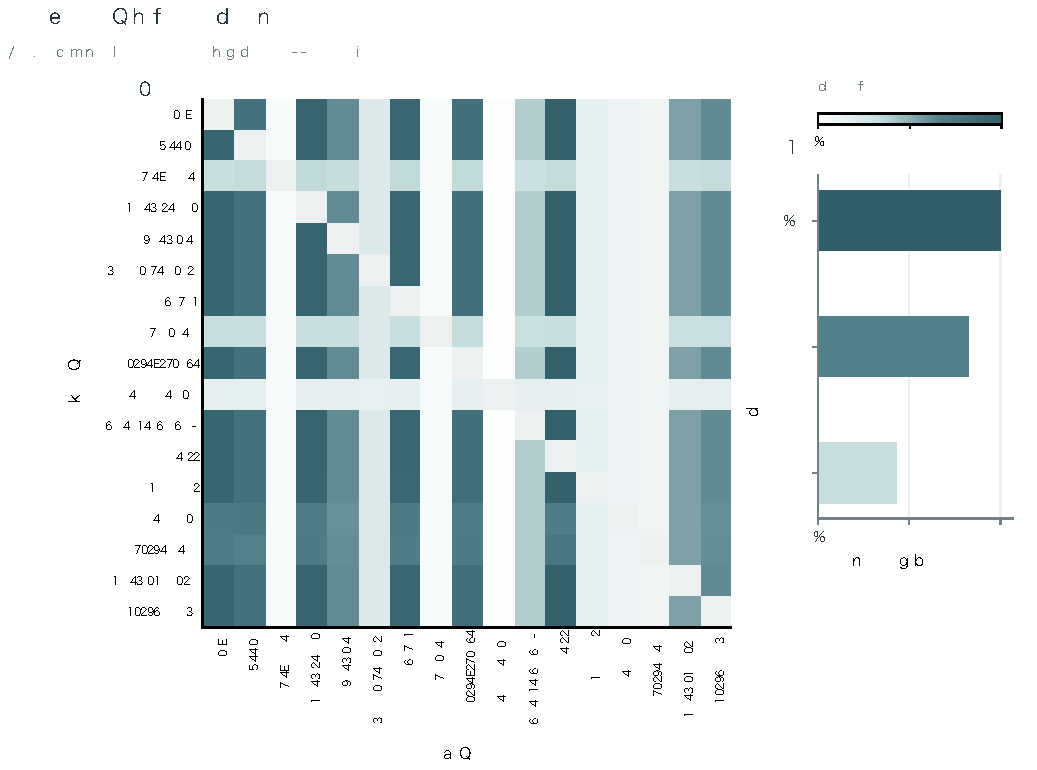
\includegraphics[width=0.96\linewidth]{figures/q3/figures/Fig01_recipe_support.pdf}
\caption{领域配方替代的凸包支持域。a 为在 99\% 安全余量下的有向替代上限，单位为百分点；b 为达到不同替代幅度的方向数。图中支持范围来自 Q2-E2，不是问题三联合模型的独立验证。}
\label{fig:q3-support}
\end{figure}

图~\ref{fig:q3-recipe-failure}比较四类配方空间。在 v1 强度下，两套质量轴于已有训练配方及其凸包中得到相同候选配方，而放开至完整单纯形后均落在纯 Enron 顶点。Enron 在 512 条训练配方中的最高占比仅为 $2.6026\%$。完整单纯形分支的 60 个资源情景全部给出负的预测 Loss，范围为 $-2.4643$ 至 $-0.9821$。非负损失指标出现负预测值表明该区域的目标函数已失去可解释性；纯 Enron 不能作为训练方案推荐，也不能用将预测值截断至零的方式掩盖问题。

\begin{figure}[htbp]
\centering
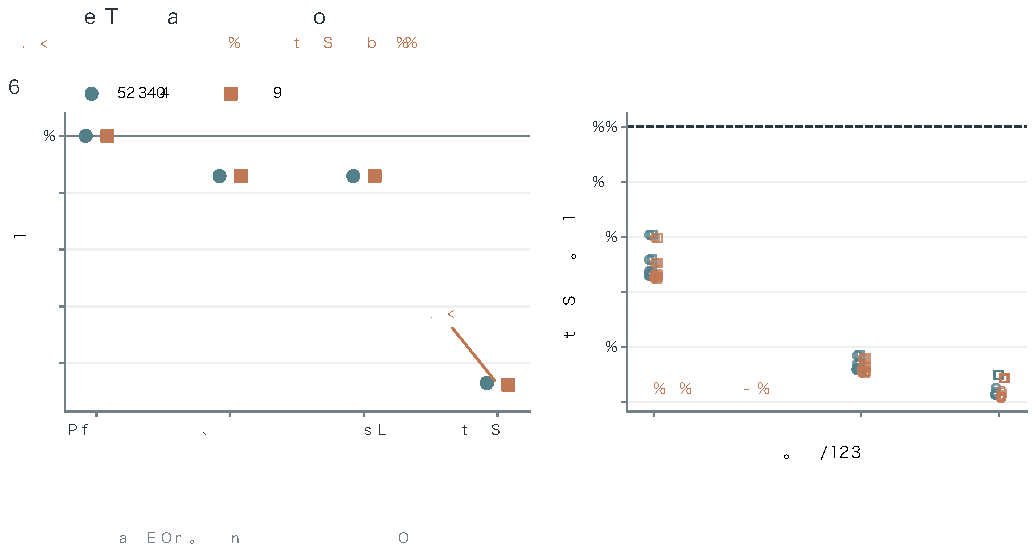
\includegraphics[width=0.96\linewidth]{figures/q3/figures/Fig02_recipe_failure.pdf}
\caption{配比可行域放开后的模型失效。a 比较参考、已有训练配方、训练凸包与完整单纯形的冻结模型修正；b 展示完整单纯形中 60 个确定性情景的负预测 Loss。横轴预算、上下文、规模边界与质量轴的组合不是独立训练重复。}
\label{fig:q3-recipe-failure}
\end{figure}

\subsection{固定配方下的质量处理与成本尺度}

为研究题面质量处理成本，额外假设配方固定后仍可提高质量坐标 $Q$，同时保持配比残差项不变。分别使用指数型 $g_1(Q)=10^7e^{6Q}$、幂型 $g_2(Q)=5\times10^9Q^4$ 和对数型 $g_3(Q)=2\times10^9\ln(1+10Q)$。处理后的预算约束为
\begin{equation}
10^{18}N_BD_B(6+\eta L_{\rm ctx})
+10^9D_B\,[g_k(Q)-g_k(Q_0)]_+\leq C,
\qquad k\in\{1,2,3\}.
\label{eq:q3-budget-process}
\end{equation}
这里 $g_k$ 按每 token 的 FLOPs 计，$10^9D_B$ 是实际 token 数。按 $Q_A$ 计价时，质量收益经 $T(Q_A)$ 进入式~\eqref{eq:q3-frozen-loss}；按 $Q_B$ 计价时，成本与收益共同使用映射后的轴。两种方案沿用相同名义参数，却代表不同成本假设；由于 $T$ 含截断，它们不是等价换元。

给定 $Q$ 后，令 $a=6+\eta L_{\rm ctx}$、$b=[g_k(Q)-g_k(Q_0)]_+/10^9$、$c=C/10^{18}$，预算边界化为 $D_B=c/(aN_B+b)$。将其代入规模项得到一维目标
\begin{equation}
F_Q(N_B)=1.689798+0.353980N_B^{-0.339977}
+1.240306\left(\frac{aN_B+b}{c}\right)^{0.279878}.
\label{eq:q3-conditional-nd}
\end{equation}
在正值可行区内由一阶条件求 $N_B$，并检查 B1 矩形边界；外层对有效质量区间以 65 点网格扫描，逐个细化局部谷值并比较端点。图~\ref{fig:q3-quality-cost}使用参考配方、$L_{\rm ctx}=2048$、指数成本、无规模上限及单位质量效应强度，展示两种评分轴和两种计价口径的 51 点对数预算扫描。按 $Q_A$ 计价的主扫描中，1530 个情景均到达各自的映射饱和上界；按 $Q_B$ 计价则出现不处理、内点与质量上界三类解。以 TOPSIS 轴为例，不处理转为内点的预算位于 $3.1623\times10^{19}$ 与 $3.9811\times10^{19}$ FLOPs 之间，内点转为上界位于 $1.5849\times10^{20}$ 与 $1.9953\times10^{20}$ FLOPs 之间。这些是步长 $0.1$ 的 $\log_{10}C$ 网格括区，不是精确阈值或经验置信区间。

\begin{figure}[htbp]
\centering
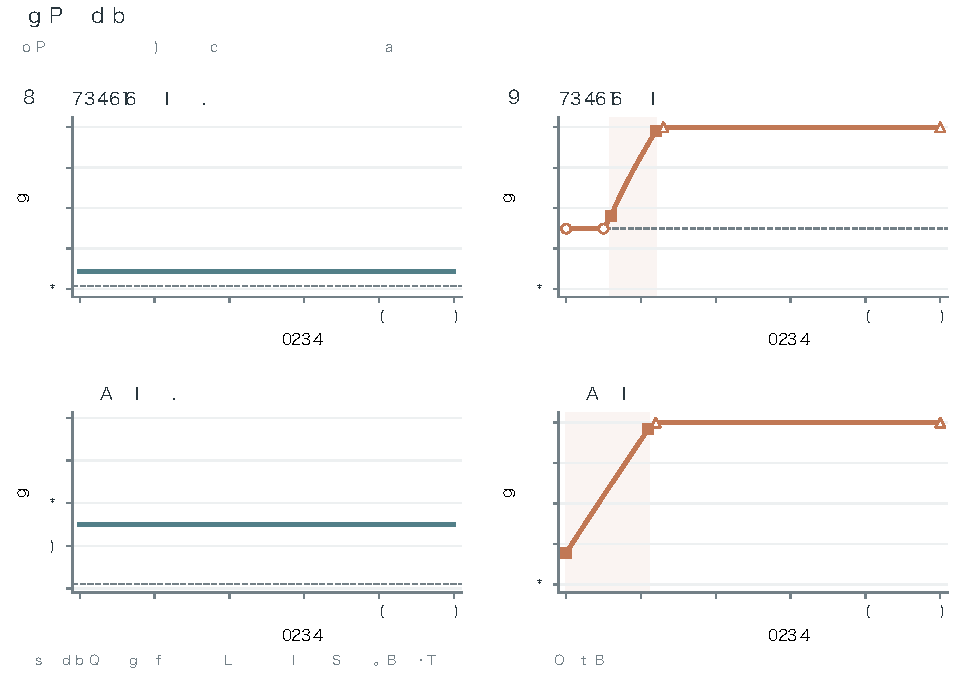
\includegraphics[width=0.96\linewidth]{figures/q3/figures/Fig03_quality_cost.pdf}
\caption{质量处理最优值对成本坐标的敏感性。a--d 分别对应 TOPSIS、soft 评分轴在 $Q_A$ 或 $Q_B$ 计价下的预算扫描；每格含 51 个确定性预算点。虚线为初始质量，阴影表示内点区间；阴影不是统计不确定性带。}
\label{fig:q3-quality-cost}
\end{figure}

表~\ref{tab:q3-cost-coordinate}固定 $C=10^{19}$ FLOPs，对照同一名义指数成本在两种质量坐标上的决策。TOPSIS 轴由映射饱和变为不处理，soft 轴则由映射饱和变为内点解；因此成本坐标的选择会改变本模型给出的处理建议。

\begin{table}[htbp]
\centering
\caption{固定参考配方、2048 上下文和指数成本下的质量处理条件解}
\label{tab:q3-cost-coordinate}
\begin{tabular}{llrrl}
\toprule
评分轴 & 成本坐标 & 初始质量 & 最优质量 & 解型 \\
\midrule
TOPSIS & $Q_A$ & 0.608376 & 0.643194 & 映射饱和 \\
TOPSIS & $Q_B$ & 0.749396 & 0.749396 & 不处理 \\
soft & $Q_A$ & 0.221428 & 0.499269 & 映射饱和 \\
soft & $Q_B$ & 0.481688 & 0.677924 & 内点 \\
\bottomrule
\end{tabular}
\end{table}

\subsection{预算配置、支持边界与决策检验}

图~\ref{fig:q3-budget-nd}给出 TOPSIS 轴、参考配方、$L_{\rm ctx}=2048$、原 v1 模型的 $N_B,D_B$ 条件配置。预算从 $10^{19}$ 增至 $10^{24}$ FLOPs 时，无规模上限解从 $(0.2213,7.0497)$ 增至 $(40.0506,3895.4695)$；在 $10^{22}$ FLOPs 时 $D_B=311.6048$ 已超过 B1 的 $299.893$ 上限。将 $N_B,D_B$ 限于 B1 矩形后，$10^{24}$ FLOPs 情景触及两个上界，预算利用率只有 $2.3001\%$。该比例说明所设可信矩形已限制模型内的扩张，不表示现实算力只能利用 $2.3001\%$。

\begin{figure}[htbp]
\centering
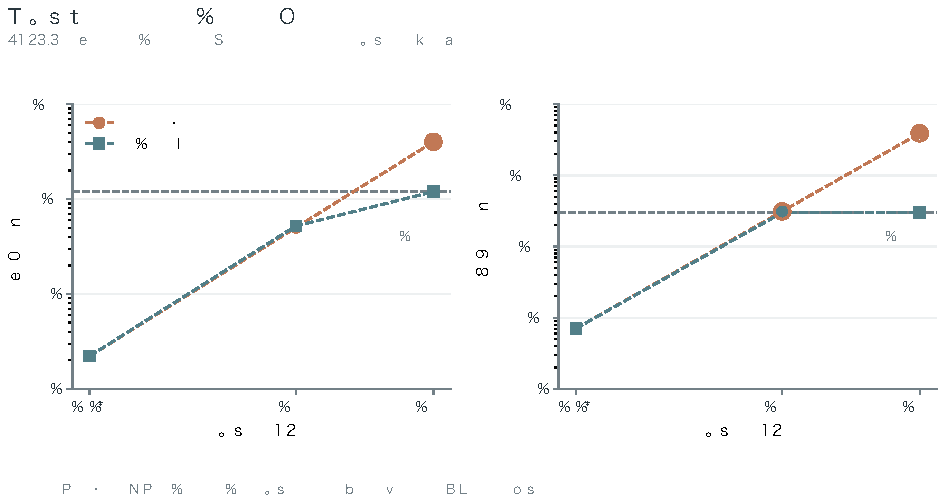
\includegraphics[width=0.94\linewidth]{figures/q3/figures/Fig04_budget_ND.pdf}
\caption{三个离散预算下的参数量和训练 token 数配置。a 为参数量 $N_B$，b 为训练 token 数 $D_B$，单位均为十亿；虚线是 B1 支持上限，空心圈表示无约束解越界。连接线仅辅助对应离散情景。}
\label{fig:q3-budget-nd}
\end{figure}

成本分解还表明，固定上下文时 $C_{\rm attn}/C_{\rm train}=\eta L_{\rm ctx}/6=L_{\rm ctx}/30000$，与预算和 $N_B,D_B$ 无关。上下文越过 $30000$ 后，注意力成本代理超过训练项；本模型未量化长上下文的任务收益，故这一成本交叉不能用于推荐最短上下文。

数值求解与决策效果应分别核对。与问题二导出的 4000 行情景比较，冻结预测的最大重建差为 $8.88\times10^{-16}$；48 个代表情景用加密质量网格和多起点全变量约束求解复核，最优目标值最大差为 $5.23\times10^{-12}$。这些是实现与求解一致性检查，不能替代对目标函数的外部预测验证。

在此前已查看的 A6、A8、A10 测试候选集合内，按冻结 v1 修正项选择预测最优配方，再读取对应实测平均 Loss。定义候选集内后悔值为
\begin{equation}
R_{\rm top1}=L_{\rm obs}(\boldsymbol p_{\rm selected})
-\min_{\boldsymbol p\in\mathcal P_{\rm test}}L_{\rm obs}(\boldsymbol p).
\label{eq:q3-regret}
\end{equation}
图~\ref{fig:q3-regret}显示 1M、60M、1B 的 $R_{\rm top1}$ 分别为 $0.7086$、$0.6179$ 和 $0.1156$ Loss，对应的实测名次是 $193/256$、$226/256$ 和 $34/64$。1M 与 60M 的配方匹配，不能视为独立重复；相关标签已进入问题二研究，因此该检验只是回溯决策诊断，不是新的盲测。

\begin{figure}[htbp]
\centering
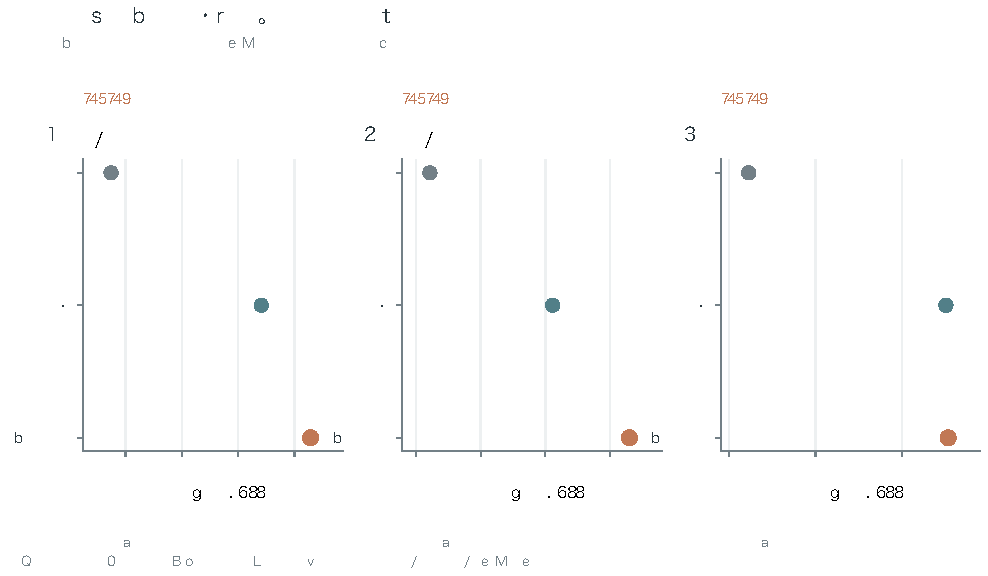
\includegraphics[width=0.96\linewidth]{figures/q3/figures/Fig05_decision_regret.pdf}
\caption{冻结 v1 在已有测试候选集内的回溯选优。三个面板分别给出候选最优、候选均值和模型选中配方的实测平均 Loss；后悔值按式~\eqref{eq:q3-regret}定义。两套质量轴在各规模选中同一配方，图中只保留一份结果。}
\label{fig:q3-regret}
\end{figure}

\subsection{结论与适用边界}

冻结条件模型的降维求解可以数值复核，但其完整单纯形最优点位于训练配方支持极弱的边界，并产生负预测 Loss；质量处理的解型又对 $Q_A$、$Q_B$ 的成本计价假设敏感。现有结果适合用于诊断资源分配机制和下一轮实验设计，尚不足以给出经验证的最优训练配方或高预算配置。下一步应先固定质量与成本的共同计量口径，限制配方可信域，再在预先留出的独立候选集上报告选优后悔值，并补充直接观测 $N,D,Q,\boldsymbol p$ 的联合训练实验。若这些证据尚未取得，本节所有数值须继续标为条件情景结果。
。
\section{问题三：冻结模型下的资源配置与可信域诊断}
\label{sec:q3-resource}

\subsection{问题分析与条件模型}

问题三要求在计算预算约束下配置模型参数量、训练数据量、数据质量与领域配比。问题二给出的损失函数含有四类变量，但现有附件缺少对四类因素的同批联合观测，因而本节将已拟合参数固定，研究该\emph{条件目标函数}的优化行为及其可信边界。首先保持质量由配比决定的原模型，再单独考察固定配比后额外处理提高质量的假设。两层情景不能混同为已经验证的四因素联合干预。

记 $N_B,D_B$ 分别为以十亿计的模型参数量和训练 token 数，$\boldsymbol p\in\Delta_{17}$ 为领域占比，$Q_A=\boldsymbol q^{\mathsf T}\boldsymbol p$ 为第一问传入的配方加权质量，$Q_B=T(Q_A)$ 为问题二冻结的截断仿射映射。采用问题二 v1 的冻结系数，有
\begin{equation}
\begin{aligned}
\widehat L(N_B,D_B,\boldsymbol p)
={}&1.689798+0.353980N_B^{-0.339977}+1.240306D_B^{-0.279878}\\
&-0.361995\lambda_Q\bigl[T(Q_A)-T(Q_{A0})\bigr]
+\lambda_p\widehat{\boldsymbol w}^{\mathsf T}\boldsymbol r(\boldsymbol p),
\end{aligned}
\label{eq:q3-frozen-loss}
\end{equation}
其中 $Q_{A0}$ 是参考配方的质量，$\boldsymbol r$ 和 $\widehat{\boldsymbol w}$ 沿用问题二的残差化定义与回归载荷；$\lambda_Q,\lambda_p$ 是预设迁移强度而非重新估计的因果系数。主情景取 $\lambda_Q=\lambda_p=1$，并以 TOPSIS 与 soft 两套评分轴检查结论对质量接口的依赖。式~\eqref{eq:q3-frozen-loss}中的数值均为模型预测，不是新增训练实验的 Loss。

设总预算为 $C$ FLOPs，上下文长度为 $L_{\rm ctx}$，题面给定的注意力系数为 $\eta=2\times10^{-4}$。在原模型中不另计提质成本，计算约束为
\begin{equation}
C_{\rm train}+C_{\rm attn}
=10^{18}N_BD_B(6+\eta L_{\rm ctx})\leq C.
\label{eq:q3-budget-original}
\end{equation}
本节考察 $C\in\{10^{19},10^{22},10^{24}\}$ 及五档上下文长度 $2048,4096,8192,32768,131072$；这些是预算与上下文情景，不是五组独立训练观测。规模可信域的矩形边界取自 B1：$N_B\in[0.070542,11.965825]$、$D_B\in[0.134,299.893]$，但矩形内的每个点并不都有联合实验支持。

\subsection{求解流程与配方支持域}

在给定质量轴及迁移强度后，配方修正项与 $N_B,D_B$ 的规模项可加分离。参考配方固定；已有 512 条训练配方直接枚举；训练配方凸包与完整 17 域单纯形上的目标，按 $T$ 的两个截断区和一个线性区分别求线性规划，再比较可行最优值。因此，原模型下同一预算和上下文的配方选择不随预算改变。这是式~\eqref{eq:q3-frozen-loss}的结构性质，不能直接推广为真实训练规律。

使用质量代理优化配比前，先检查训练配方覆盖的局部替代方向。图~\ref{fig:q3-support}显示，17 域构成的 272 个有向替代在 0.1 个百分点阈值下均有有限支持；达到 1 个和 5 个百分点的方向分别为 224 个和 117 个。该支持域来自问题二 E2 的训练配方凸包与 99\% 安全余量，只能说明几何可构造性，不能说明相应替代已接受实际训练验证。

\begin{figure}[htbp]
\centering
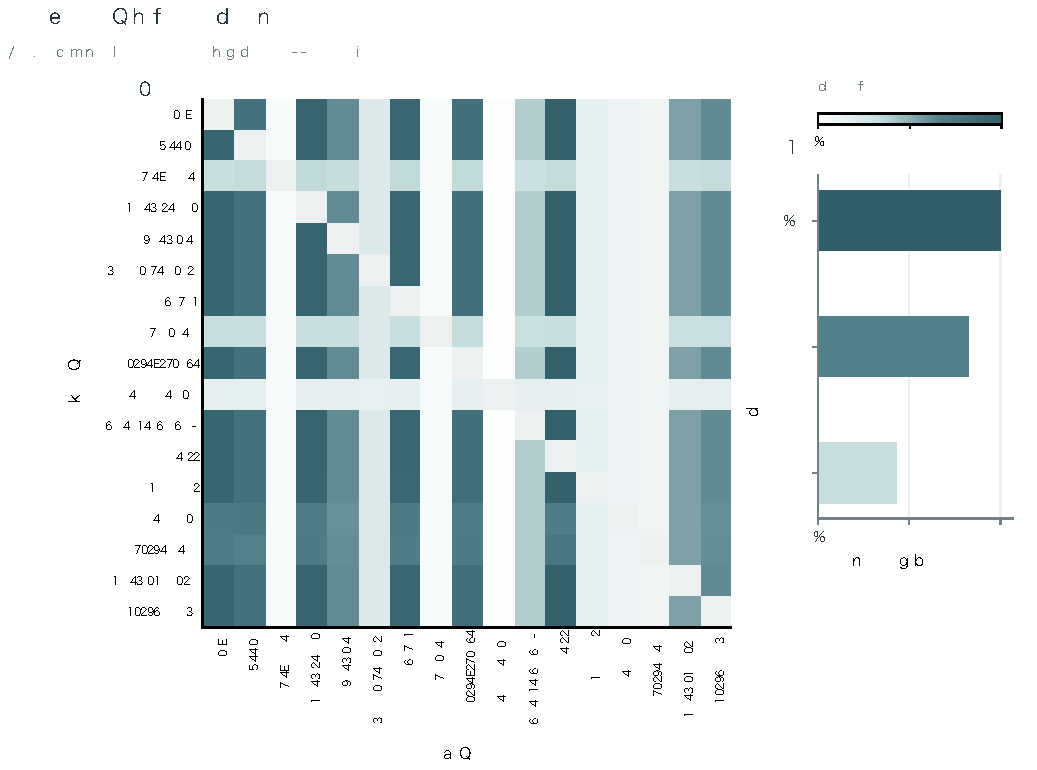
\includegraphics[width=0.96\linewidth]{figures/q3/figures/Fig01_recipe_support.pdf}
\caption{领域配方替代的凸包支持域。a 为在 99\% 安全余量下的有向替代上限，单位为百分点；b 为达到不同替代幅度的方向数。图中支持范围来自 Q2-E2，不是问题三联合模型的独立验证。}
\label{fig:q3-support}
\end{figure}

图~\ref{fig:q3-recipe-failure}比较四类配方空间。在 v1 强度下，两套质量轴于已有训练配方及其凸包中得到相同候选配方，而放开至完整单纯形后均落在纯 Enron 顶点。Enron 在 512 条训练配方中的最高占比仅为 $2.6026\%$。完整单纯形分支的 60 个资源情景全部给出负的预测 Loss，范围为 $-2.4643$ 至 $-0.9821$。非负损失指标出现负预测值表明该区域的目标函数已失去可解释性；纯 Enron 不能作为训练方案推荐，也不能用将预测值截断至零的方式掩盖问题。

\begin{figure}[htbp]
\centering
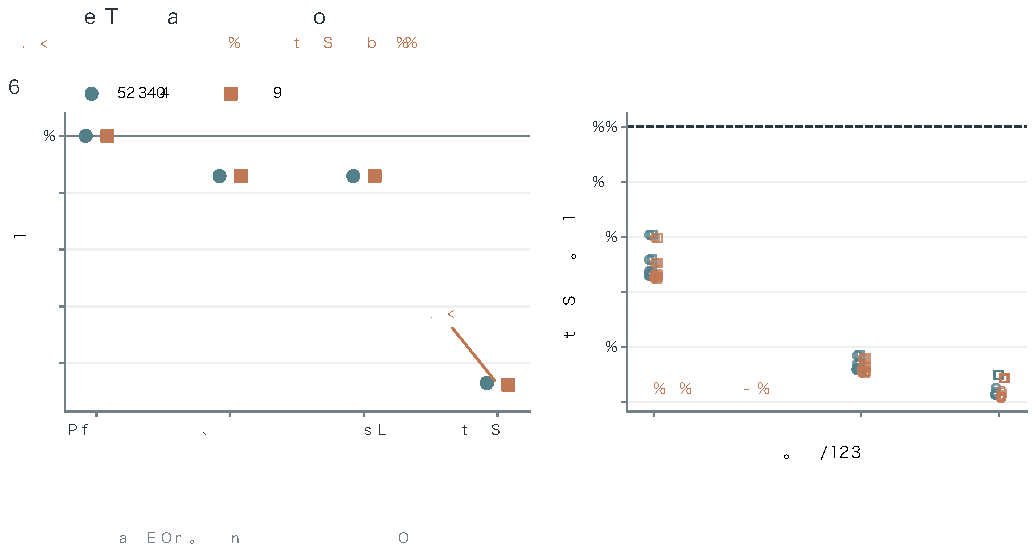
\includegraphics[width=0.96\linewidth]{figures/q3/figures/Fig02_recipe_failure.pdf}
\caption{配比可行域放开后的模型失效。a 比较参考、已有训练配方、训练凸包与完整单纯形的冻结模型修正；b 展示完整单纯形中 60 个确定性情景的负预测 Loss。横轴预算、上下文、规模边界与质量轴的组合不是独立训练重复。}
\label{fig:q3-recipe-failure}
\end{figure}

\subsection{固定配方下的质量处理与成本尺度}

为研究题面质量处理成本，额外假设配方固定后仍可提高质量坐标 $Q$，同时保持配比残差项不变。分别使用指数型 $g_1(Q)=10^7e^{6Q}$、幂型 $g_2(Q)=5\times10^9Q^4$ 和对数型 $g_3(Q)=2\times10^9\ln(1+10Q)$。处理后的预算约束为
\begin{equation}
10^{18}N_BD_B(6+\eta L_{\rm ctx})
+10^9D_B\,[g_k(Q)-g_k(Q_0)]_+\leq C,
\qquad k\in\{1,2,3\}.
\label{eq:q3-budget-process}
\end{equation}
这里 $g_k$ 按每 token 的 FLOPs 计，$10^9D_B$ 是实际 token 数。按 $Q_A$ 计价时，质量收益经 $T(Q_A)$ 进入式~\eqref{eq:q3-frozen-loss}；按 $Q_B$ 计价时，成本与收益共同使用映射后的轴。两种方案沿用相同名义参数，却代表不同成本假设；由于 $T$ 含截断，它们不是等价换元。

给定 $Q$ 后，令 $a=6+\eta L_{\rm ctx}$、$b=[g_k(Q)-g_k(Q_0)]_+/10^9$、$c=C/10^{18}$，预算边界化为 $D_B=c/(aN_B+b)$。将其代入规模项得到一维目标
\begin{equation}
F_Q(N_B)=1.689798+0.353980N_B^{-0.339977}
+1.240306\left(\frac{aN_B+b}{c}\right)^{0.279878}.
\label{eq:q3-conditional-nd}
\end{equation}
在正值可行区内由一阶条件求 $N_B$，并检查 B1 矩形边界；外层对有效质量区间以 65 点网格扫描，逐个细化局部谷值并比较端点。图~\ref{fig:q3-quality-cost}使用参考配方、$L_{\rm ctx}=2048$、指数成本、无规模上限及单位质量效应强度，展示两种评分轴和两种计价口径的 51 点对数预算扫描。按 $Q_A$ 计价的主扫描中，1530 个情景均到达各自的映射饱和上界；按 $Q_B$ 计价则出现不处理、内点与质量上界三类解。以 TOPSIS 轴为例，不处理转为内点的预算位于 $3.1623\times10^{19}$ 与 $3.9811\times10^{19}$ FLOPs 之间，内点转为上界位于 $1.5849\times10^{20}$ 与 $1.9953\times10^{20}$ FLOPs 之间。这些是步长 $0.1$ 的 $\log_{10}C$ 网格括区，不是精确阈值或经验置信区间。

\begin{figure}[htbp]
\centering
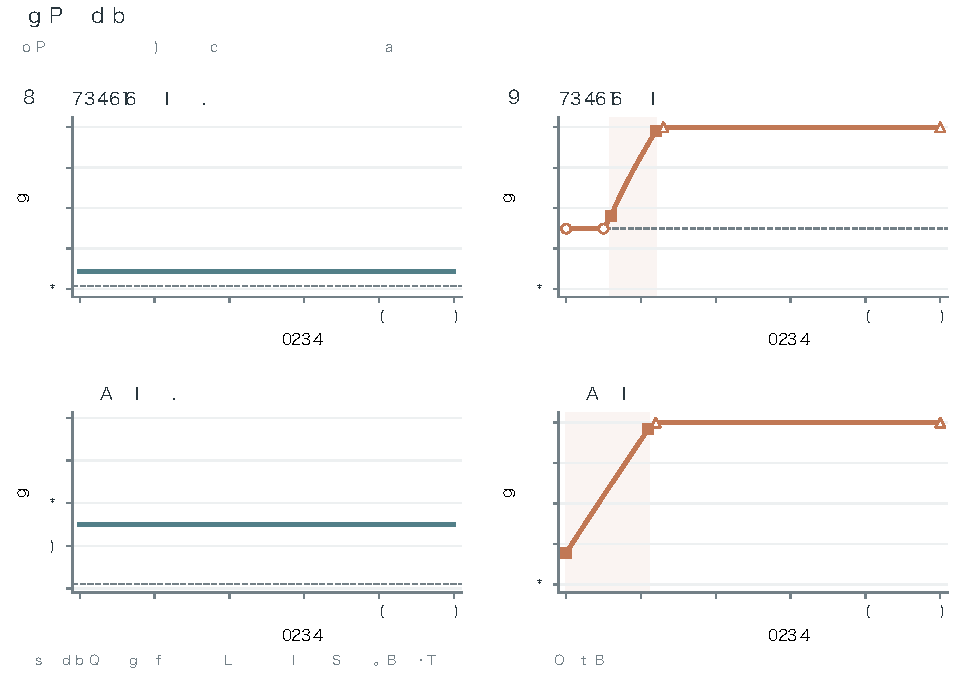
\includegraphics[width=0.96\linewidth]{figures/q3/figures/Fig03_quality_cost.pdf}
\caption{质量处理最优值对成本坐标的敏感性。a--d 分别对应 TOPSIS、soft 评分轴在 $Q_A$ 或 $Q_B$ 计价下的预算扫描；每格含 51 个确定性预算点。虚线为初始质量，阴影表示内点区间；阴影不是统计不确定性带。}
\label{fig:q3-quality-cost}
\end{figure}

表~\ref{tab:q3-cost-coordinate}固定 $C=10^{19}$ FLOPs，对照同一名义指数成本在两种质量坐标上的决策。TOPSIS 轴由映射饱和变为不处理，soft 轴则由映射饱和变为内点解；因此成本坐标的选择会改变本模型给出的处理建议。

\begin{table}[htbp]
\centering
\caption{固定参考配方、2048 上下文和指数成本下的质量处理条件解}
\label{tab:q3-cost-coordinate}
\begin{tabular}{llrrl}
\toprule
评分轴 & 成本坐标 & 初始质量 & 最优质量 & 解型 \\
\midrule
TOPSIS & $Q_A$ & 0.608376 & 0.643194 & 映射饱和 \\
TOPSIS & $Q_B$ & 0.749396 & 0.749396 & 不处理 \\
soft & $Q_A$ & 0.221428 & 0.499269 & 映射饱和 \\
soft & $Q_B$ & 0.481688 & 0.677924 & 内点 \\
\bottomrule
\end{tabular}
\end{table}

\subsection{预算配置、支持边界与决策检验}

图~\ref{fig:q3-budget-nd}给出 TOPSIS 轴、参考配方、$L_{\rm ctx}=2048$、原 v1 模型的 $N_B,D_B$ 条件配置。预算从 $10^{19}$ 增至 $10^{24}$ FLOPs 时，无规模上限解从 $(0.2213,7.0497)$ 增至 $(40.0506,3895.4695)$；在 $10^{22}$ FLOPs 时 $D_B=311.6048$ 已超过 B1 的 $299.893$ 上限。将 $N_B,D_B$ 限于 B1 矩形后，$10^{24}$ FLOPs 情景触及两个上界，预算利用率只有 $2.3001\%$。该比例说明所设可信矩形已限制模型内的扩张，不表示现实算力只能利用 $2.3001\%$。

\begin{figure}[htbp]
\centering
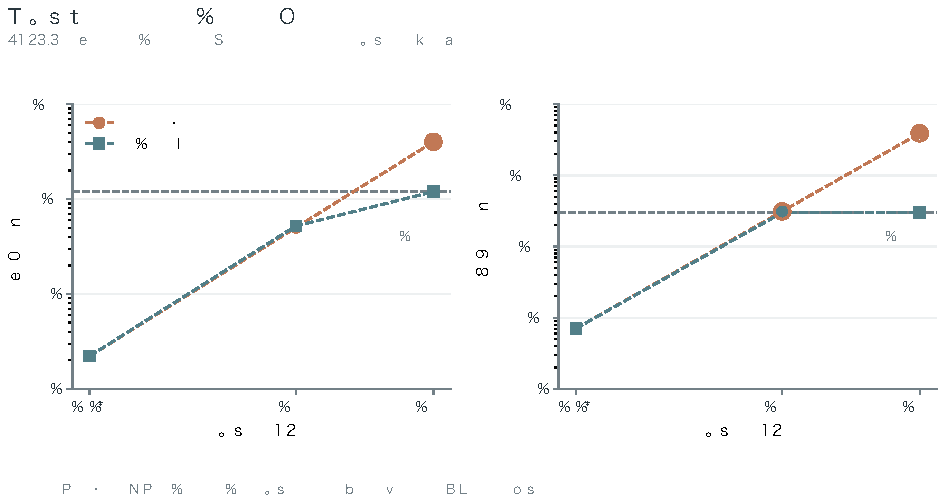
\includegraphics[width=0.94\linewidth]{figures/q3/figures/Fig04_budget_ND.pdf}
\caption{三个离散预算下的参数量和训练 token 数配置。a 为参数量 $N_B$，b 为训练 token 数 $D_B$，单位均为十亿；虚线是 B1 支持上限，空心圈表示无约束解越界。连接线仅辅助对应离散情景。}
\label{fig:q3-budget-nd}
\end{figure}

成本分解还表明，固定上下文时 $C_{\rm attn}/C_{\rm train}=\eta L_{\rm ctx}/6=L_{\rm ctx}/30000$，与预算和 $N_B,D_B$ 无关。上下文越过 $30000$ 后，注意力成本代理超过训练项；本模型未量化长上下文的任务收益，故这一成本交叉不能用于推荐最短上下文。

数值求解与决策效果应分别核对。与问题二导出的 4000 行情景比较，冻结预测的最大重建差为 $8.88\times10^{-16}$；48 个代表情景用加密质量网格和多起点全变量约束求解复核，最优目标值最大差为 $5.23\times10^{-12}$。这些是实现与求解一致性检查，不能替代对目标函数的外部预测验证。

在此前已查看的 A6、A8、A10 测试候选集合内，按冻结 v1 修正项选择预测最优配方，再读取对应实测平均 Loss。定义候选集内后悔值为
\begin{equation}
R_{\rm top1}=L_{\rm obs}(\boldsymbol p_{\rm selected})
-\min_{\boldsymbol p\in\mathcal P_{\rm test}}L_{\rm obs}(\boldsymbol p).
\label{eq:q3-regret}
\end{equation}
图~\ref{fig:q3-regret}显示 1M、60M、1B 的 $R_{\rm top1}$ 分别为 $0.7086$、$0.6179$ 和 $0.1156$ Loss，对应的实测名次是 $193/256$、$226/256$ 和 $34/64$。1M 与 60M 的配方匹配，不能视为独立重复；相关标签已进入问题二研究，因此该检验只是回溯决策诊断，不是新的盲测。

\begin{figure}[htbp]
\centering
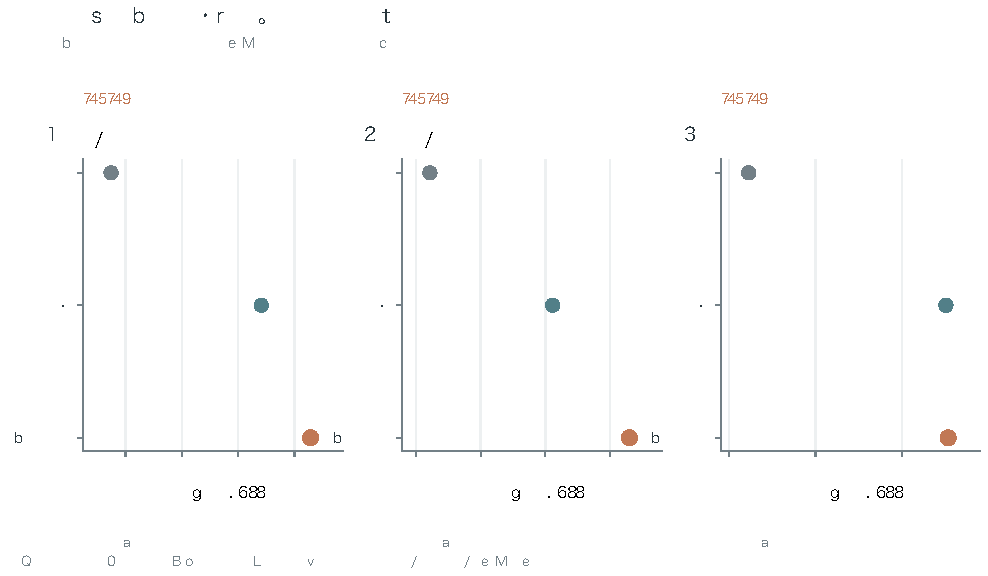
\includegraphics[width=0.96\linewidth]{figures/q3/figures/Fig05_decision_regret.pdf}
\caption{冻结 v1 在已有测试候选集内的回溯选优。三个面板分别给出候选最优、候选均值和模型选中配方的实测平均 Loss；后悔值按式~\eqref{eq:q3-regret}定义。两套质量轴在各规模选中同一配方，图中只保留一份结果。}
\label{fig:q3-regret}
\end{figure}

\subsection{结论与适用边界}

冻结条件模型的降维求解可以数值复核，但其完整单纯形最优点位于训练配方支持极弱的边界，并产生负预测 Loss；质量处理的解型又对 $Q_A$、$Q_B$ 的成本计价假设敏感。现有结果适合用于诊断资源分配机制和下一轮实验设计，尚不足以给出经验证的最优训练配方或高预算配置。下一步应先固定质量与成本的共同计量口径，限制配方可信域，再在预先留出的独立候选集上报告选优后悔值，并补充直接观测 $N,D,Q,\boldsymbol p$ 的联合训练实验。若这些证据尚未取得，本节所有数值须继续标为条件情景结果。
。
\section{问题三：冻结模型下的资源配置与可信域诊断}
\label{sec:q3-resource}

\subsection{问题分析与条件模型}

问题三要求在计算预算约束下配置模型参数量、训练数据量、数据质量与领域配比。问题二给出的损失函数含有四类变量，但现有附件缺少对四类因素的同批联合观测，因而本节将已拟合参数固定，研究该\emph{条件目标函数}的优化行为及其可信边界。首先保持质量由配比决定的原模型，再单独考察固定配比后额外处理提高质量的假设。两层情景不能混同为已经验证的四因素联合干预。

记 $N_B,D_B$ 分别为以十亿计的模型参数量和训练 token 数，$\boldsymbol p\in\Delta_{17}$ 为领域占比，$Q_A=\boldsymbol q^{\mathsf T}\boldsymbol p$ 为第一问传入的配方加权质量，$Q_B=T(Q_A)$ 为问题二冻结的截断仿射映射。采用问题二 v1 的冻结系数，有
\begin{equation}
\begin{aligned}
\widehat L(N_B,D_B,\boldsymbol p)
={}&1.689798+0.353980N_B^{-0.339977}+1.240306D_B^{-0.279878}\\
&-0.361995\lambda_Q\bigl[T(Q_A)-T(Q_{A0})\bigr]
+\lambda_p\widehat{\boldsymbol w}^{\mathsf T}\boldsymbol r(\boldsymbol p),
\end{aligned}
\label{eq:q3-frozen-loss}
\end{equation}
其中 $Q_{A0}$ 是参考配方的质量，$\boldsymbol r$ 和 $\widehat{\boldsymbol w}$ 沿用问题二的残差化定义与回归载荷；$\lambda_Q,\lambda_p$ 是预设迁移强度而非重新估计的因果系数。主情景取 $\lambda_Q=\lambda_p=1$，并以 TOPSIS 与 soft 两套评分轴检查结论对质量接口的依赖。式~\eqref{eq:q3-frozen-loss}中的数值均为模型预测，不是新增训练实验的 Loss。

设总预算为 $C$ FLOPs，上下文长度为 $L_{\rm ctx}$，题面给定的注意力系数为 $\eta=2\times10^{-4}$。在原模型中不另计提质成本，计算约束为
\begin{equation}
C_{\rm train}+C_{\rm attn}
=10^{18}N_BD_B(6+\eta L_{\rm ctx})\leq C.
\label{eq:q3-budget-original}
\end{equation}
本节考察 $C\in\{10^{19},10^{22},10^{24}\}$ 及五档上下文长度 $2048,4096,8192,32768,131072$；这些是预算与上下文情景，不是五组独立训练观测。规模可信域的矩形边界取自 B1：$N_B\in[0.070542,11.965825]$、$D_B\in[0.134,299.893]$，但矩形内的每个点并不都有联合实验支持。

\subsection{求解流程与配方支持域}

在给定质量轴及迁移强度后，配方修正项与 $N_B,D_B$ 的规模项可加分离。参考配方固定；已有 512 条训练配方直接枚举；训练配方凸包与完整 17 域单纯形上的目标，按 $T$ 的两个截断区和一个线性区分别求线性规划，再比较可行最优值。因此，原模型下同一预算和上下文的配方选择不随预算改变。这是式~\eqref{eq:q3-frozen-loss}的结构性质，不能直接推广为真实训练规律。

使用质量代理优化配比前，先检查训练配方覆盖的局部替代方向。图~\ref{fig:q3-support}显示，17 域构成的 272 个有向替代在 0.1 个百分点阈值下均有有限支持；达到 1 个和 5 个百分点的方向分别为 224 个和 117 个。该支持域来自问题二 E2 的训练配方凸包与 99\% 安全余量，只能说明几何可构造性，不能说明相应替代已接受实际训练验证。

\begin{figure}[htbp]
\centering
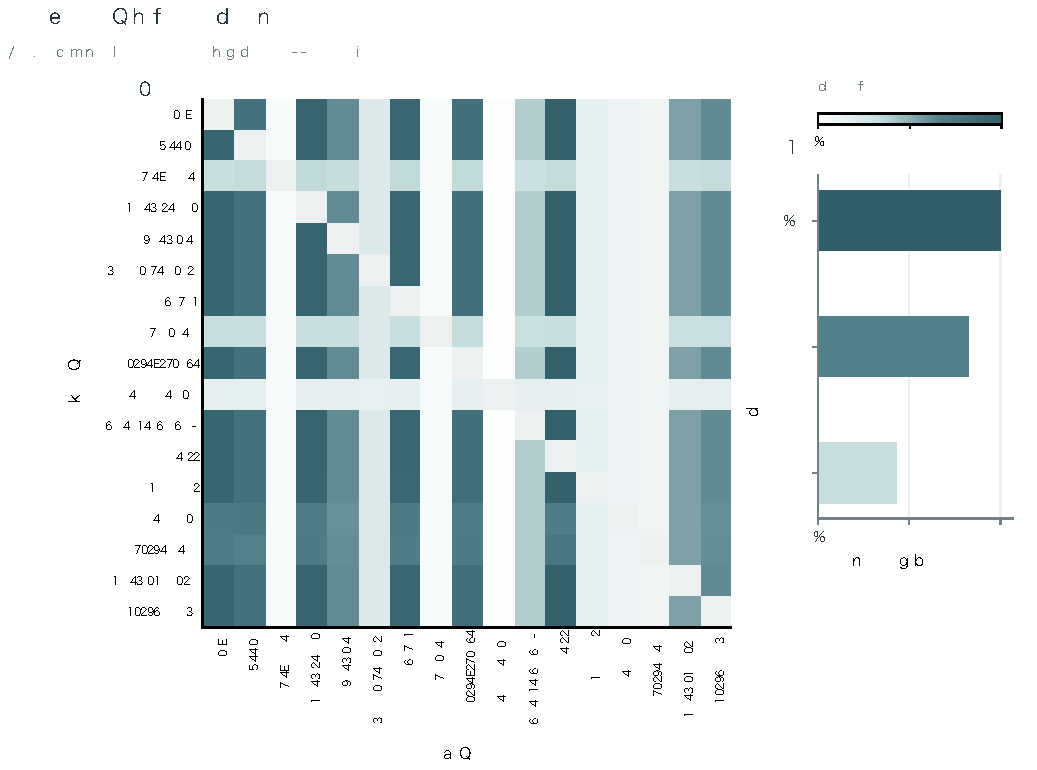
\includegraphics[width=0.96\linewidth]{figures/q3/figures/Fig01_recipe_support.pdf}
\caption{领域配方替代的凸包支持域。a 为在 99\% 安全余量下的有向替代上限，单位为百分点；b 为达到不同替代幅度的方向数。图中支持范围来自 Q2-E2，不是问题三联合模型的独立验证。}
\label{fig:q3-support}
\end{figure}

图~\ref{fig:q3-recipe-failure}比较四类配方空间。在 v1 强度下，两套质量轴于已有训练配方及其凸包中得到相同候选配方，而放开至完整单纯形后均落在纯 Enron 顶点。Enron 在 512 条训练配方中的最高占比仅为 $2.6026\%$。完整单纯形分支的 60 个资源情景全部给出负的预测 Loss，范围为 $-2.4643$ 至 $-0.9821$。非负损失指标出现负预测值表明该区域的目标函数已失去可解释性；纯 Enron 不能作为训练方案推荐，也不能用将预测值截断至零的方式掩盖问题。

\begin{figure}[htbp]
\centering
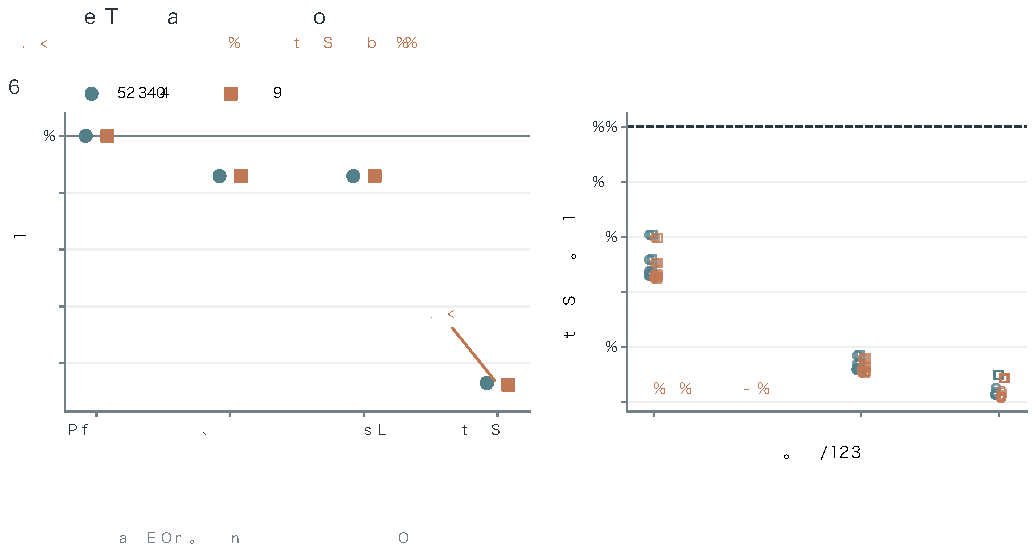
\includegraphics[width=0.96\linewidth]{figures/q3/figures/Fig02_recipe_failure.pdf}
\caption{配比可行域放开后的模型失效。a 比较参考、已有训练配方、训练凸包与完整单纯形的冻结模型修正；b 展示完整单纯形中 60 个确定性情景的负预测 Loss。横轴预算、上下文、规模边界与质量轴的组合不是独立训练重复。}
\label{fig:q3-recipe-failure}
\end{figure}

\subsection{固定配方下的质量处理与成本尺度}

为研究题面质量处理成本，额外假设配方固定后仍可提高质量坐标 $Q$，同时保持配比残差项不变。分别使用指数型 $g_1(Q)=10^7e^{6Q}$、幂型 $g_2(Q)=5\times10^9Q^4$ 和对数型 $g_3(Q)=2\times10^9\ln(1+10Q)$。处理后的预算约束为
\begin{equation}
10^{18}N_BD_B(6+\eta L_{\rm ctx})
+10^9D_B\,[g_k(Q)-g_k(Q_0)]_+\leq C,
\qquad k\in\{1,2,3\}.
\label{eq:q3-budget-process}
\end{equation}
这里 $g_k$ 按每 token 的 FLOPs 计，$10^9D_B$ 是实际 token 数。按 $Q_A$ 计价时，质量收益经 $T(Q_A)$ 进入式~\eqref{eq:q3-frozen-loss}；按 $Q_B$ 计价时，成本与收益共同使用映射后的轴。两种方案沿用相同名义参数，却代表不同成本假设；由于 $T$ 含截断，它们不是等价换元。

给定 $Q$ 后，令 $a=6+\eta L_{\rm ctx}$、$b=[g_k(Q)-g_k(Q_0)]_+/10^9$、$c=C/10^{18}$，预算边界化为 $D_B=c/(aN_B+b)$。将其代入规模项得到一维目标
\begin{equation}
F_Q(N_B)=1.689798+0.353980N_B^{-0.339977}
+1.240306\left(\frac{aN_B+b}{c}\right)^{0.279878}.
\label{eq:q3-conditional-nd}
\end{equation}
在正值可行区内由一阶条件求 $N_B$，并检查 B1 矩形边界；外层对有效质量区间以 65 点网格扫描，逐个细化局部谷值并比较端点。图~\ref{fig:q3-quality-cost}使用参考配方、$L_{\rm ctx}=2048$、指数成本、无规模上限及单位质量效应强度，展示两种评分轴和两种计价口径的 51 点对数预算扫描。按 $Q_A$ 计价的主扫描中，1530 个情景均到达各自的映射饱和上界；按 $Q_B$ 计价则出现不处理、内点与质量上界三类解。以 TOPSIS 轴为例，不处理转为内点的预算位于 $3.1623\times10^{19}$ 与 $3.9811\times10^{19}$ FLOPs 之间，内点转为上界位于 $1.5849\times10^{20}$ 与 $1.9953\times10^{20}$ FLOPs 之间。这些是步长 $0.1$ 的 $\log_{10}C$ 网格括区，不是精确阈值或经验置信区间。

\begin{figure}[htbp]
\centering
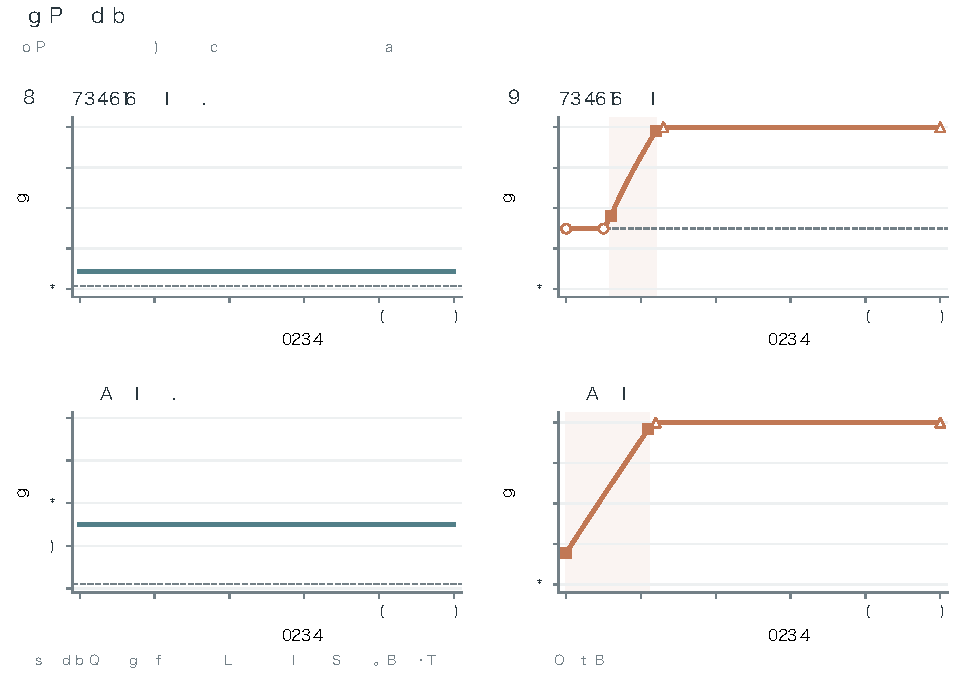
\includegraphics[width=0.96\linewidth]{figures/q3/figures/Fig03_quality_cost.pdf}
\caption{质量处理最优值对成本坐标的敏感性。a--d 分别对应 TOPSIS、soft 评分轴在 $Q_A$ 或 $Q_B$ 计价下的预算扫描；每格含 51 个确定性预算点。虚线为初始质量，阴影表示内点区间；阴影不是统计不确定性带。}
\label{fig:q3-quality-cost}
\end{figure}

表~\ref{tab:q3-cost-coordinate}固定 $C=10^{19}$ FLOPs，对照同一名义指数成本在两种质量坐标上的决策。TOPSIS 轴由映射饱和变为不处理，soft 轴则由映射饱和变为内点解；因此成本坐标的选择会改变本模型给出的处理建议。

\begin{table}[htbp]
\centering
\caption{固定参考配方、2048 上下文和指数成本下的质量处理条件解}
\label{tab:q3-cost-coordinate}
\begin{tabular}{llrrl}
\toprule
评分轴 & 成本坐标 & 初始质量 & 最优质量 & 解型 \\
\midrule
TOPSIS & $Q_A$ & 0.608376 & 0.643194 & 映射饱和 \\
TOPSIS & $Q_B$ & 0.749396 & 0.749396 & 不处理 \\
soft & $Q_A$ & 0.221428 & 0.499269 & 映射饱和 \\
soft & $Q_B$ & 0.481688 & 0.677924 & 内点 \\
\bottomrule
\end{tabular}
\end{table}

\subsection{预算配置、支持边界与决策检验}

图~\ref{fig:q3-budget-nd}给出 TOPSIS 轴、参考配方、$L_{\rm ctx}=2048$、原 v1 模型的 $N_B,D_B$ 条件配置。预算从 $10^{19}$ 增至 $10^{24}$ FLOPs 时，无规模上限解从 $(0.2213,7.0497)$ 增至 $(40.0506,3895.4695)$；在 $10^{22}$ FLOPs 时 $D_B=311.6048$ 已超过 B1 的 $299.893$ 上限。将 $N_B,D_B$ 限于 B1 矩形后，$10^{24}$ FLOPs 情景触及两个上界，预算利用率只有 $2.3001\%$。该比例说明所设可信矩形已限制模型内的扩张，不表示现实算力只能利用 $2.3001\%$。

\begin{figure}[htbp]
\centering
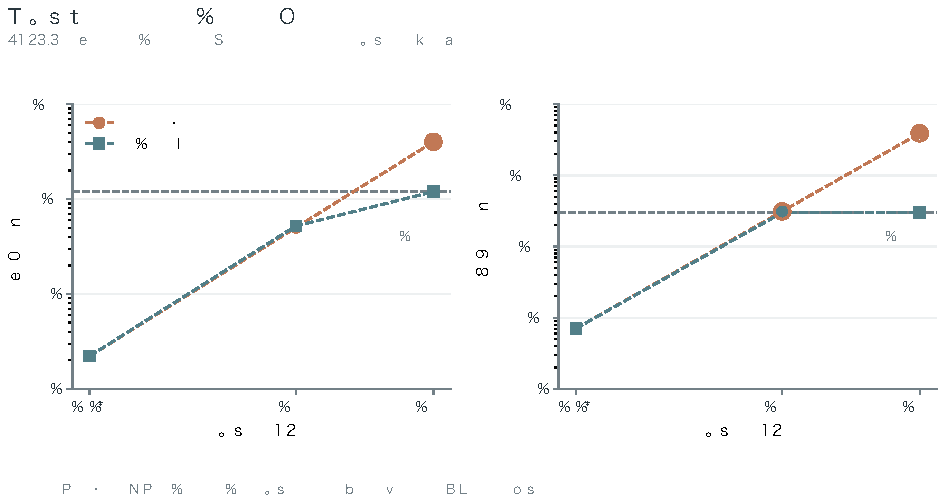
\includegraphics[width=0.94\linewidth]{figures/q3/figures/Fig04_budget_ND.pdf}
\caption{三个离散预算下的参数量和训练 token 数配置。a 为参数量 $N_B$，b 为训练 token 数 $D_B$，单位均为十亿；虚线是 B1 支持上限，空心圈表示无约束解越界。连接线仅辅助对应离散情景。}
\label{fig:q3-budget-nd}
\end{figure}

成本分解还表明，固定上下文时 $C_{\rm attn}/C_{\rm train}=\eta L_{\rm ctx}/6=L_{\rm ctx}/30000$，与预算和 $N_B,D_B$ 无关。上下文越过 $30000$ 后，注意力成本代理超过训练项；本模型未量化长上下文的任务收益，故这一成本交叉不能用于推荐最短上下文。

数值求解与决策效果应分别核对。与问题二导出的 4000 行情景比较，冻结预测的最大重建差为 $8.88\times10^{-16}$；48 个代表情景用加密质量网格和多起点全变量约束求解复核，最优目标值最大差为 $5.23\times10^{-12}$。这些是实现与求解一致性检查，不能替代对目标函数的外部预测验证。

在此前已查看的 A6、A8、A10 测试候选集合内，按冻结 v1 修正项选择预测最优配方，再读取对应实测平均 Loss。定义候选集内后悔值为
\begin{equation}
R_{\rm top1}=L_{\rm obs}(\boldsymbol p_{\rm selected})
-\min_{\boldsymbol p\in\mathcal P_{\rm test}}L_{\rm obs}(\boldsymbol p).
\label{eq:q3-regret}
\end{equation}
图~\ref{fig:q3-regret}显示 1M、60M、1B 的 $R_{\rm top1}$ 分别为 $0.7086$、$0.6179$ 和 $0.1156$ Loss，对应的实测名次是 $193/256$、$226/256$ 和 $34/64$。1M 与 60M 的配方匹配，不能视为独立重复；相关标签已进入问题二研究，因此该检验只是回溯决策诊断，不是新的盲测。

\begin{figure}[htbp]
\centering
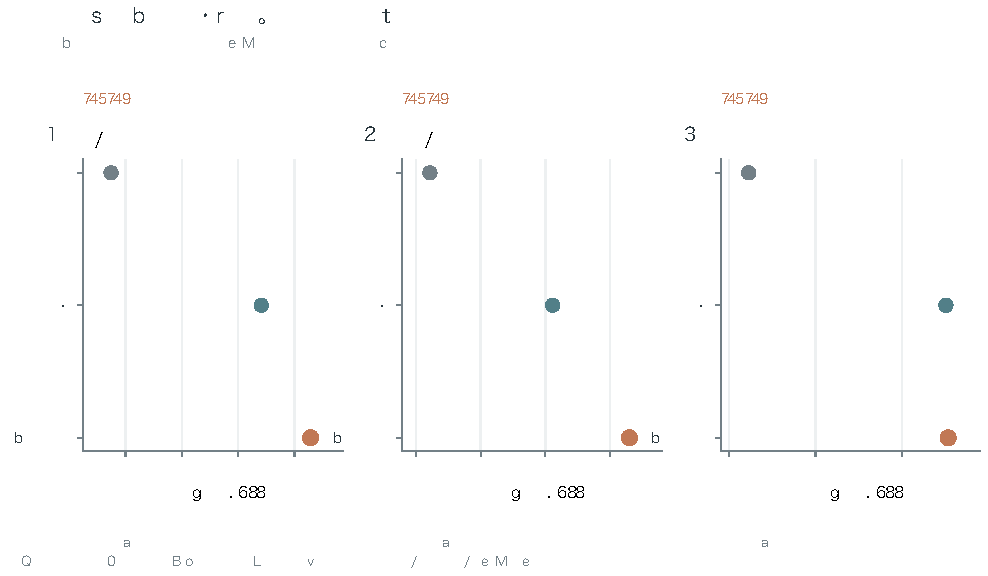
\includegraphics[width=0.96\linewidth]{figures/q3/figures/Fig05_decision_regret.pdf}
\caption{冻结 v1 在已有测试候选集内的回溯选优。三个面板分别给出候选最优、候选均值和模型选中配方的实测平均 Loss；后悔值按式~\eqref{eq:q3-regret}定义。两套质量轴在各规模选中同一配方，图中只保留一份结果。}
\label{fig:q3-regret}
\end{figure}

\subsection{结论与适用边界}

冻结条件模型的降维求解可以数值复核，但其完整单纯形最优点位于训练配方支持极弱的边界，并产生负预测 Loss；质量处理的解型又对 $Q_A$、$Q_B$ 的成本计价假设敏感。现有结果适合用于诊断资源分配机制和下一轮实验设计，尚不足以给出经验证的最优训练配方或高预算配置。下一步应先固定质量与成本的共同计量口径，限制配方可信域，再在预先留出的独立候选集上报告选优后悔值，并补充直接观测 $N,D,Q,\boldsymbol p$ 的联合训练实验。若这些证据尚未取得，本节所有数值须继续标为条件情景结果。
。
\section{问题三：冻结模型下的资源配置与可信域诊断}
\label{sec:q3-resource}

\subsection{问题分析与条件模型}

问题三要求在计算预算约束下配置模型参数量、训练数据量、数据质量与领域配比。问题二给出的损失函数含有四类变量，但现有附件缺少对四类因素的同批联合观测，因而本节将已拟合参数固定，研究该\emph{条件目标函数}的优化行为及其可信边界。首先保持质量由配比决定的原模型，再单独考察固定配比后额外处理提高质量的假设。两层情景不能混同为已经验证的四因素联合干预。

记 $N_B,D_B$ 分别为以十亿计的模型参数量和训练 token 数，$\boldsymbol p\in\Delta_{17}$ 为领域占比，$Q_A=\boldsymbol q^{\mathsf T}\boldsymbol p$ 为第一问传入的配方加权质量，$Q_B=T(Q_A)$ 为问题二冻结的截断仿射映射。采用问题二 v1 的冻结系数，有
\begin{equation}
\begin{aligned}
\widehat L(N_B,D_B,\boldsymbol p)
={}&1.689798+0.353980N_B^{-0.339977}+1.240306D_B^{-0.279878}\\
&-0.361995\lambda_Q\bigl[T(Q_A)-T(Q_{A0})\bigr]
+\lambda_p\widehat{\boldsymbol w}^{\mathsf T}\boldsymbol r(\boldsymbol p),
\end{aligned}
\label{eq:q3-frozen-loss}
\end{equation}
其中 $Q_{A0}$ 是参考配方的质量，$\boldsymbol r$ 和 $\widehat{\boldsymbol w}$ 沿用问题二的残差化定义与回归载荷；$\lambda_Q,\lambda_p$ 是预设迁移强度而非重新估计的因果系数。主情景取 $\lambda_Q=\lambda_p=1$，并以 TOPSIS 与 soft 两套评分轴检查结论对质量接口的依赖。式~\eqref{eq:q3-frozen-loss}中的数值均为模型预测，不是新增训练实验的 Loss。

设总预算为 $C$ FLOPs，上下文长度为 $L_{\rm ctx}$，题面给定的注意力系数为 $\eta=2\times10^{-4}$。在原模型中不另计提质成本，计算约束为
\begin{equation}
C_{\rm train}+C_{\rm attn}
=10^{18}N_BD_B(6+\eta L_{\rm ctx})\leq C.
\label{eq:q3-budget-original}
\end{equation}
本节考察 $C\in\{10^{19},10^{22},10^{24}\}$ 及五档上下文长度 $2048,4096,8192,32768,131072$；这些是预算与上下文情景，不是五组独立训练观测。规模可信域的矩形边界取自 B1：$N_B\in[0.070542,11.965825]$、$D_B\in[0.134,299.893]$，但矩形内的每个点并不都有联合实验支持。

\subsection{求解流程与配方支持域}

在给定质量轴及迁移强度后，配方修正项与 $N_B,D_B$ 的规模项可加分离。参考配方固定；已有 512 条训练配方直接枚举；训练配方凸包与完整 17 域单纯形上的目标，按 $T$ 的两个截断区和一个线性区分别求线性规划，再比较可行最优值。因此，原模型下同一预算和上下文的配方选择不随预算改变。这是式~\eqref{eq:q3-frozen-loss}的结构性质，不能直接推广为真实训练规律。

使用质量代理优化配比前，先检查训练配方覆盖的局部替代方向。图~\ref{fig:q3-support}显示，17 域构成的 272 个有向替代在 0.1 个百分点阈值下均有有限支持；达到 1 个和 5 个百分点的方向分别为 224 个和 117 个。该支持域来自问题二 E2 的训练配方凸包与 99\% 安全余量，只能说明几何可构造性，不能说明相应替代已接受实际训练验证。

\begin{figure}[htbp]
\centering
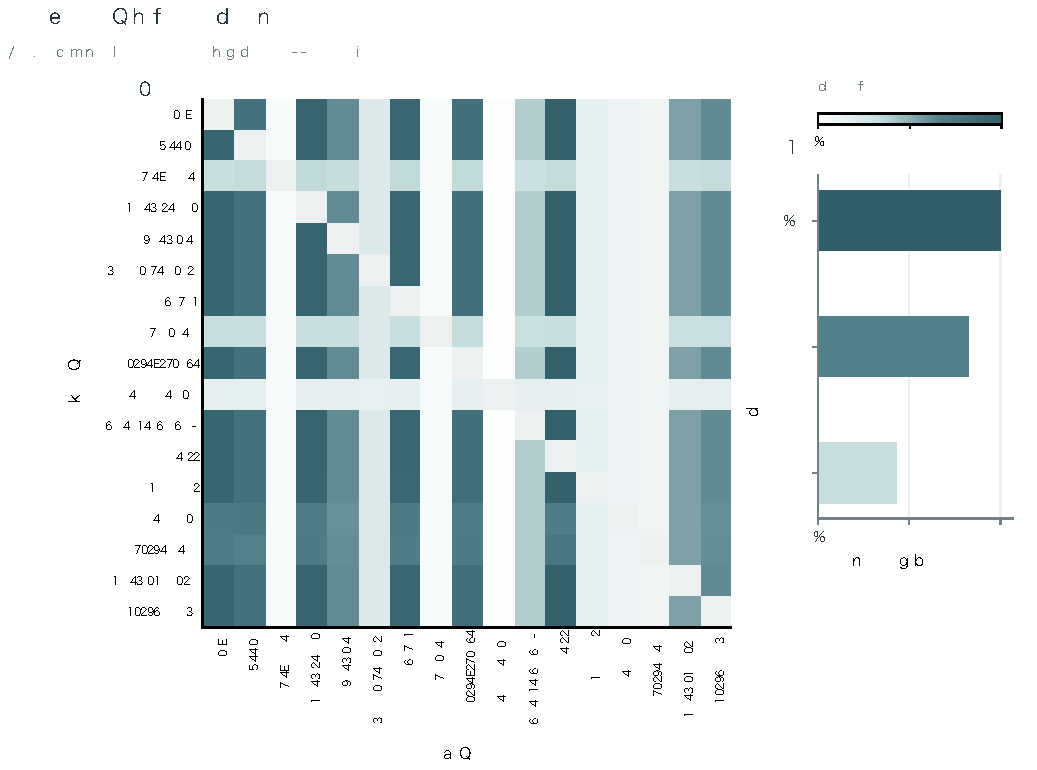
\includegraphics[width=0.96\linewidth]{figures/q3/figures/Fig01_recipe_support.pdf}
\caption{领域配方替代的凸包支持域。a 为在 99\% 安全余量下的有向替代上限，单位为百分点；b 为达到不同替代幅度的方向数。图中支持范围来自 Q2-E2，不是问题三联合模型的独立验证。}
\label{fig:q3-support}
\end{figure}

图~\ref{fig:q3-recipe-failure}比较四类配方空间。在 v1 强度下，两套质量轴于已有训练配方及其凸包中得到相同候选配方，而放开至完整单纯形后均落在纯 Enron 顶点。Enron 在 512 条训练配方中的最高占比仅为 $2.6026\%$。完整单纯形分支的 60 个资源情景全部给出负的预测 Loss，范围为 $-2.4643$ 至 $-0.9821$。非负损失指标出现负预测值表明该区域的目标函数已失去可解释性；纯 Enron 不能作为训练方案推荐，也不能用将预测值截断至零的方式掩盖问题。

\begin{figure}[htbp]
\centering
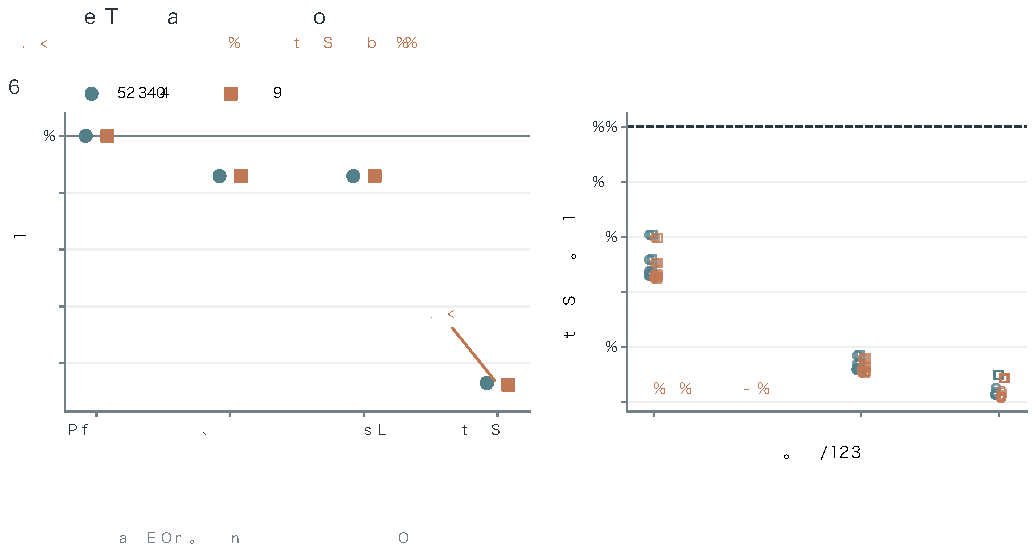
\includegraphics[width=0.96\linewidth]{figures/q3/figures/Fig02_recipe_failure.pdf}
\caption{配比可行域放开后的模型失效。a 比较参考、已有训练配方、训练凸包与完整单纯形的冻结模型修正；b 展示完整单纯形中 60 个确定性情景的负预测 Loss。横轴预算、上下文、规模边界与质量轴的组合不是独立训练重复。}
\label{fig:q3-recipe-failure}
\end{figure}

\subsection{固定配方下的质量处理与成本尺度}

为研究题面质量处理成本，额外假设配方固定后仍可提高质量坐标 $Q$，同时保持配比残差项不变。分别使用指数型 $g_1(Q)=10^7e^{6Q}$、幂型 $g_2(Q)=5\times10^9Q^4$ 和对数型 $g_3(Q)=2\times10^9\ln(1+10Q)$。处理后的预算约束为
\begin{equation}
10^{18}N_BD_B(6+\eta L_{\rm ctx})
+10^9D_B\,[g_k(Q)-g_k(Q_0)]_+\leq C,
\qquad k\in\{1,2,3\}.
\label{eq:q3-budget-process}
\end{equation}
这里 $g_k$ 按每 token 的 FLOPs 计，$10^9D_B$ 是实际 token 数。按 $Q_A$ 计价时，质量收益经 $T(Q_A)$ 进入式~\eqref{eq:q3-frozen-loss}；按 $Q_B$ 计价时，成本与收益共同使用映射后的轴。两种方案沿用相同名义参数，却代表不同成本假设；由于 $T$ 含截断，它们不是等价换元。

给定 $Q$ 后，令 $a=6+\eta L_{\rm ctx}$、$b=[g_k(Q)-g_k(Q_0)]_+/10^9$、$c=C/10^{18}$，预算边界化为 $D_B=c/(aN_B+b)$。将其代入规模项得到一维目标
\begin{equation}
F_Q(N_B)=1.689798+0.353980N_B^{-0.339977}
+1.240306\left(\frac{aN_B+b}{c}\right)^{0.279878}.
\label{eq:q3-conditional-nd}
\end{equation}
在正值可行区内由一阶条件求 $N_B$，并检查 B1 矩形边界；外层对有效质量区间以 65 点网格扫描，逐个细化局部谷值并比较端点。图~\ref{fig:q3-quality-cost}使用参考配方、$L_{\rm ctx}=2048$、指数成本、无规模上限及单位质量效应强度，展示两种评分轴和两种计价口径的 51 点对数预算扫描。按 $Q_A$ 计价的主扫描中，1530 个情景均到达各自的映射饱和上界；按 $Q_B$ 计价则出现不处理、内点与质量上界三类解。以 TOPSIS 轴为例，不处理转为内点的预算位于 $3.1623\times10^{19}$ 与 $3.9811\times10^{19}$ FLOPs 之间，内点转为上界位于 $1.5849\times10^{20}$ 与 $1.9953\times10^{20}$ FLOPs 之间。这些是步长 $0.1$ 的 $\log_{10}C$ 网格括区，不是精确阈值或经验置信区间。

\begin{figure}[htbp]
\centering
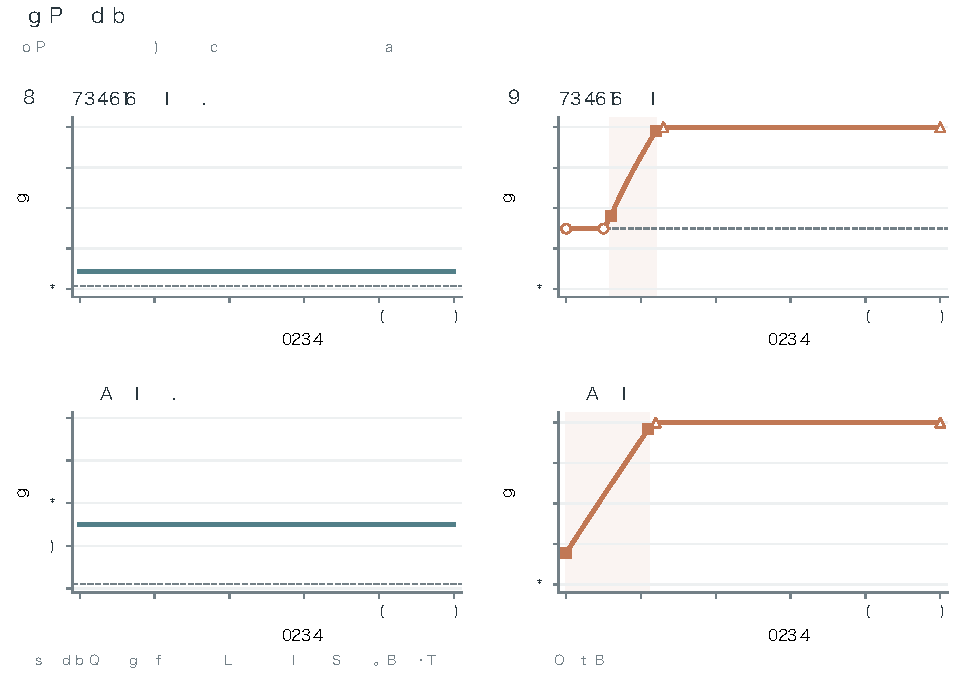
\includegraphics[width=0.96\linewidth]{figures/q3/figures/Fig03_quality_cost.pdf}
\caption{质量处理最优值对成本坐标的敏感性。a--d 分别对应 TOPSIS、soft 评分轴在 $Q_A$ 或 $Q_B$ 计价下的预算扫描；每格含 51 个确定性预算点。虚线为初始质量，阴影表示内点区间；阴影不是统计不确定性带。}
\label{fig:q3-quality-cost}
\end{figure}

表~\ref{tab:q3-cost-coordinate}固定 $C=10^{19}$ FLOPs，对照同一名义指数成本在两种质量坐标上的决策。TOPSIS 轴由映射饱和变为不处理，soft 轴则由映射饱和变为内点解；因此成本坐标的选择会改变本模型给出的处理建议。

\begin{table}[htbp]
\centering
\caption{固定参考配方、2048 上下文和指数成本下的质量处理条件解}
\label{tab:q3-cost-coordinate}
\begin{tabular}{llrrl}
\toprule
评分轴 & 成本坐标 & 初始质量 & 最优质量 & 解型 \\
\midrule
TOPSIS & $Q_A$ & 0.608376 & 0.643194 & 映射饱和 \\
TOPSIS & $Q_B$ & 0.749396 & 0.749396 & 不处理 \\
soft & $Q_A$ & 0.221428 & 0.499269 & 映射饱和 \\
soft & $Q_B$ & 0.481688 & 0.677924 & 内点 \\
\bottomrule
\end{tabular}
\end{table}

\subsection{预算配置、支持边界与决策检验}

图~\ref{fig:q3-budget-nd}给出 TOPSIS 轴、参考配方、$L_{\rm ctx}=2048$、原 v1 模型的 $N_B,D_B$ 条件配置。预算从 $10^{19}$ 增至 $10^{24}$ FLOPs 时，无规模上限解从 $(0.2213,7.0497)$ 增至 $(40.0506,3895.4695)$；在 $10^{22}$ FLOPs 时 $D_B=311.6048$ 已超过 B1 的 $299.893$ 上限。将 $N_B,D_B$ 限于 B1 矩形后，$10^{24}$ FLOPs 情景触及两个上界，预算利用率只有 $2.3001\%$。该比例说明所设可信矩形已限制模型内的扩张，不表示现实算力只能利用 $2.3001\%$。

\begin{figure}[htbp]
\centering
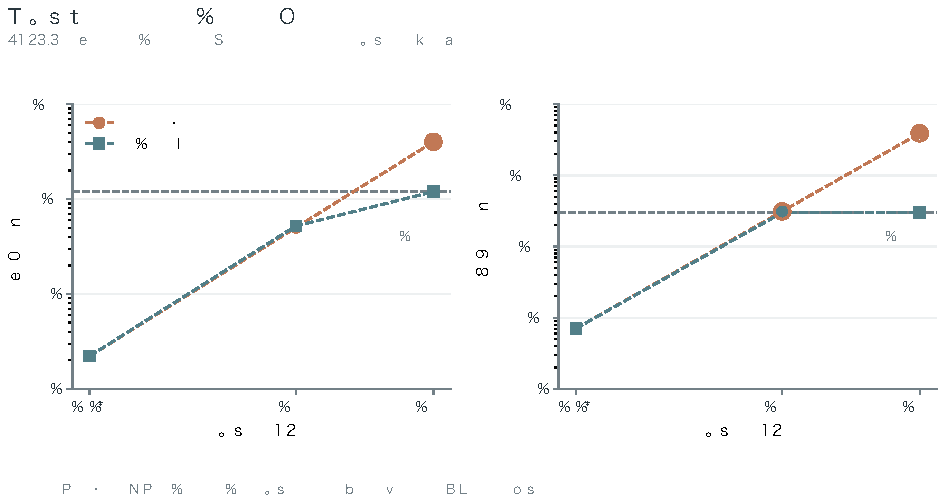
\includegraphics[width=0.94\linewidth]{figures/q3/figures/Fig04_budget_ND.pdf}
\caption{三个离散预算下的参数量和训练 token 数配置。a 为参数量 $N_B$，b 为训练 token 数 $D_B$，单位均为十亿；虚线是 B1 支持上限，空心圈表示无约束解越界。连接线仅辅助对应离散情景。}
\label{fig:q3-budget-nd}
\end{figure}

成本分解还表明，固定上下文时 $C_{\rm attn}/C_{\rm train}=\eta L_{\rm ctx}/6=L_{\rm ctx}/30000$，与预算和 $N_B,D_B$ 无关。上下文越过 $30000$ 后，注意力成本代理超过训练项；本模型未量化长上下文的任务收益，故这一成本交叉不能用于推荐最短上下文。

数值求解与决策效果应分别核对。与问题二导出的 4000 行情景比较，冻结预测的最大重建差为 $8.88\times10^{-16}$；48 个代表情景用加密质量网格和多起点全变量约束求解复核，最优目标值最大差为 $5.23\times10^{-12}$。这些是实现与求解一致性检查，不能替代对目标函数的外部预测验证。

在此前已查看的 A6、A8、A10 测试候选集合内，按冻结 v1 修正项选择预测最优配方，再读取对应实测平均 Loss。定义候选集内后悔值为
\begin{equation}
R_{\rm top1}=L_{\rm obs}(\boldsymbol p_{\rm selected})
-\min_{\boldsymbol p\in\mathcal P_{\rm test}}L_{\rm obs}(\boldsymbol p).
\label{eq:q3-regret}
\end{equation}
图~\ref{fig:q3-regret}显示 1M、60M、1B 的 $R_{\rm top1}$ 分别为 $0.7086$、$0.6179$ 和 $0.1156$ Loss，对应的实测名次是 $193/256$、$226/256$ 和 $34/64$。1M 与 60M 的配方匹配，不能视为独立重复；相关标签已进入问题二研究，因此该检验只是回溯决策诊断，不是新的盲测。

\begin{figure}[htbp]
\centering
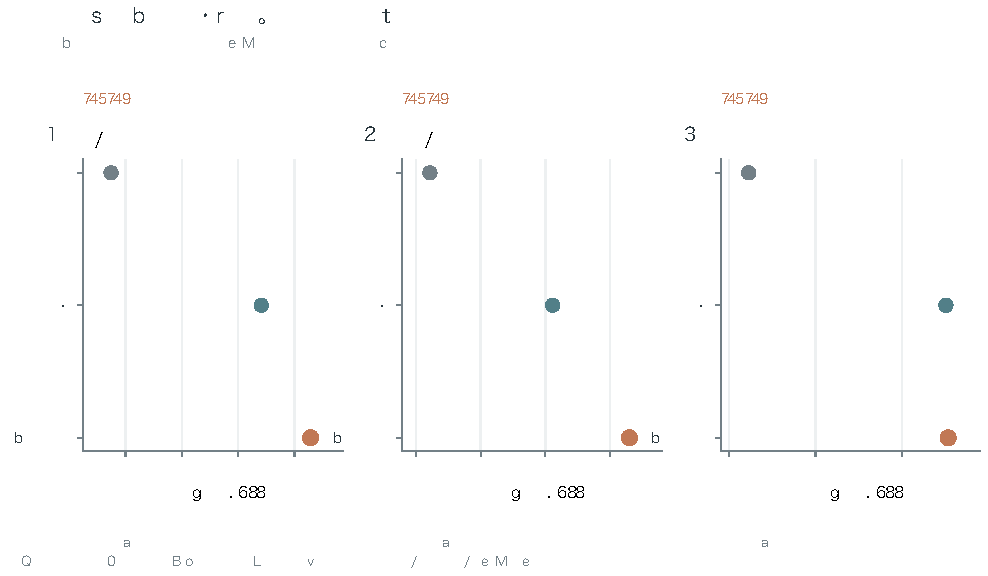
\includegraphics[width=0.96\linewidth]{figures/q3/figures/Fig05_decision_regret.pdf}
\caption{冻结 v1 在已有测试候选集内的回溯选优。三个面板分别给出候选最优、候选均值和模型选中配方的实测平均 Loss；后悔值按式~\eqref{eq:q3-regret}定义。两套质量轴在各规模选中同一配方，图中只保留一份结果。}
\label{fig:q3-regret}
\end{figure}

\subsection{结论与适用边界}

冻结条件模型的降维求解可以数值复核，但其完整单纯形最优点位于训练配方支持极弱的边界，并产生负预测 Loss；质量处理的解型又对 $Q_A$、$Q_B$ 的成本计价假设敏感。现有结果适合用于诊断资源分配机制和下一轮实验设计，尚不足以给出经验证的最优训练配方或高预算配置。下一步应先固定质量与成本的共同计量口径，限制配方可信域，再在预先留出的独立候选集上报告选优后悔值，并补充直接观测 $N,D,Q,\boldsymbol p$ 的联合训练实验。若这些证据尚未取得，本节所有数值须继续标为条件情景结果。
